\chapter{ギルバート乗算回路}
    \section{回路構成}
        まず、図\ref{fig:2_gilbert}に現在広く使用されているギルバート乗算回路の回路図を示す。
        \begin{figure}[bth]
            \begin{center}
                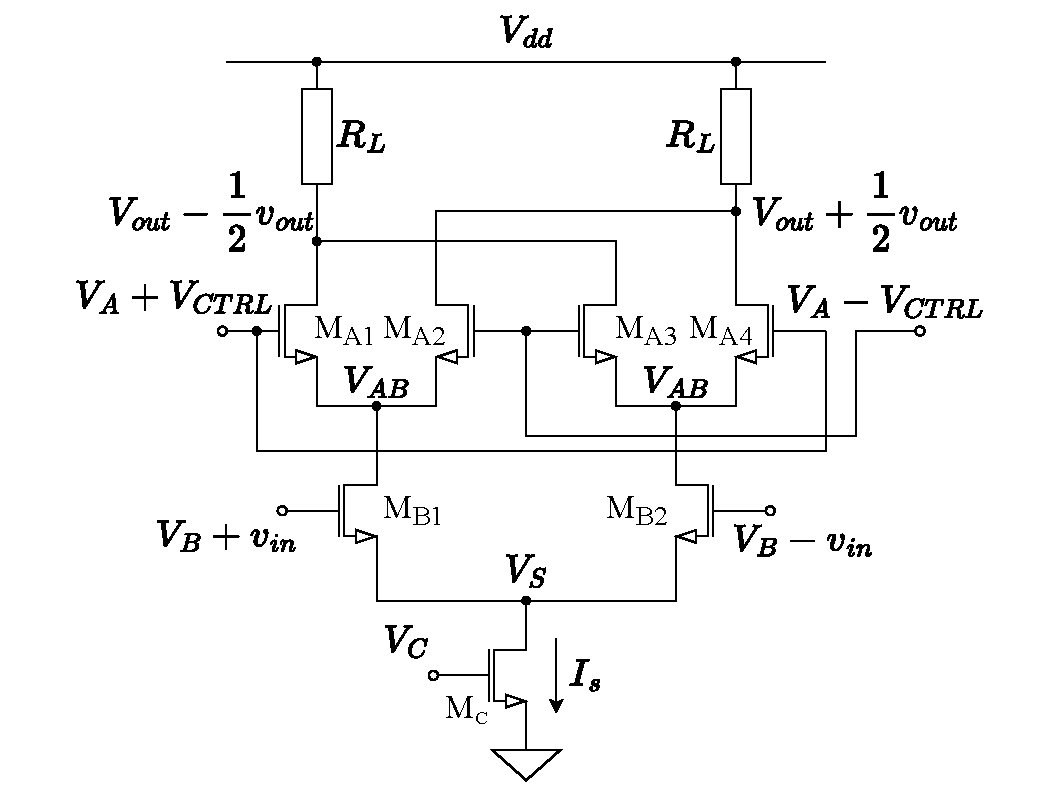
\includegraphics[width=0.99\textwidth]{figures/chapter2/gilbert.pdf}
                \caption{ギルバート乗算回路}
                \label{fig:2_gilbert}
            \end{center}
        \end{figure}
        ギルバート乗算回路は$v_{in}$と$V_{CTRL}$に差動で信号を入力することで二つの入力信号に比例した電圧出力を差動で出力することができる。ここで、$M_{B}$の差動対は入力信号に比例した電流を$M_{A}$のソースから引き込む。さらに$M_{A}$の動作点が制御電圧$V_{CTRL}$に比例して変動することに注意すると負荷抵抗に流れる電流が二つの入力に比例していることが分かる。詳細は次節にて導出する。


    \section{小信号解析}
        \subsection{動作点の変動}   \label{ch:gilbert_valiable_gm}
            小信号解析を行うにあたり$M_{A}$の扱いが問題となる。小信号解析ではMOSFETの出力が線形に近似できるような小信号入力に対して行うが、動作点が変動すると線形な近似が合わなくなる。この問題を扱うために、まず図\ref{fig:2_OP}に示す差動ゲート接地の差動対について考える。\par
            \begin{figure}[b]
                \begin{center}
                    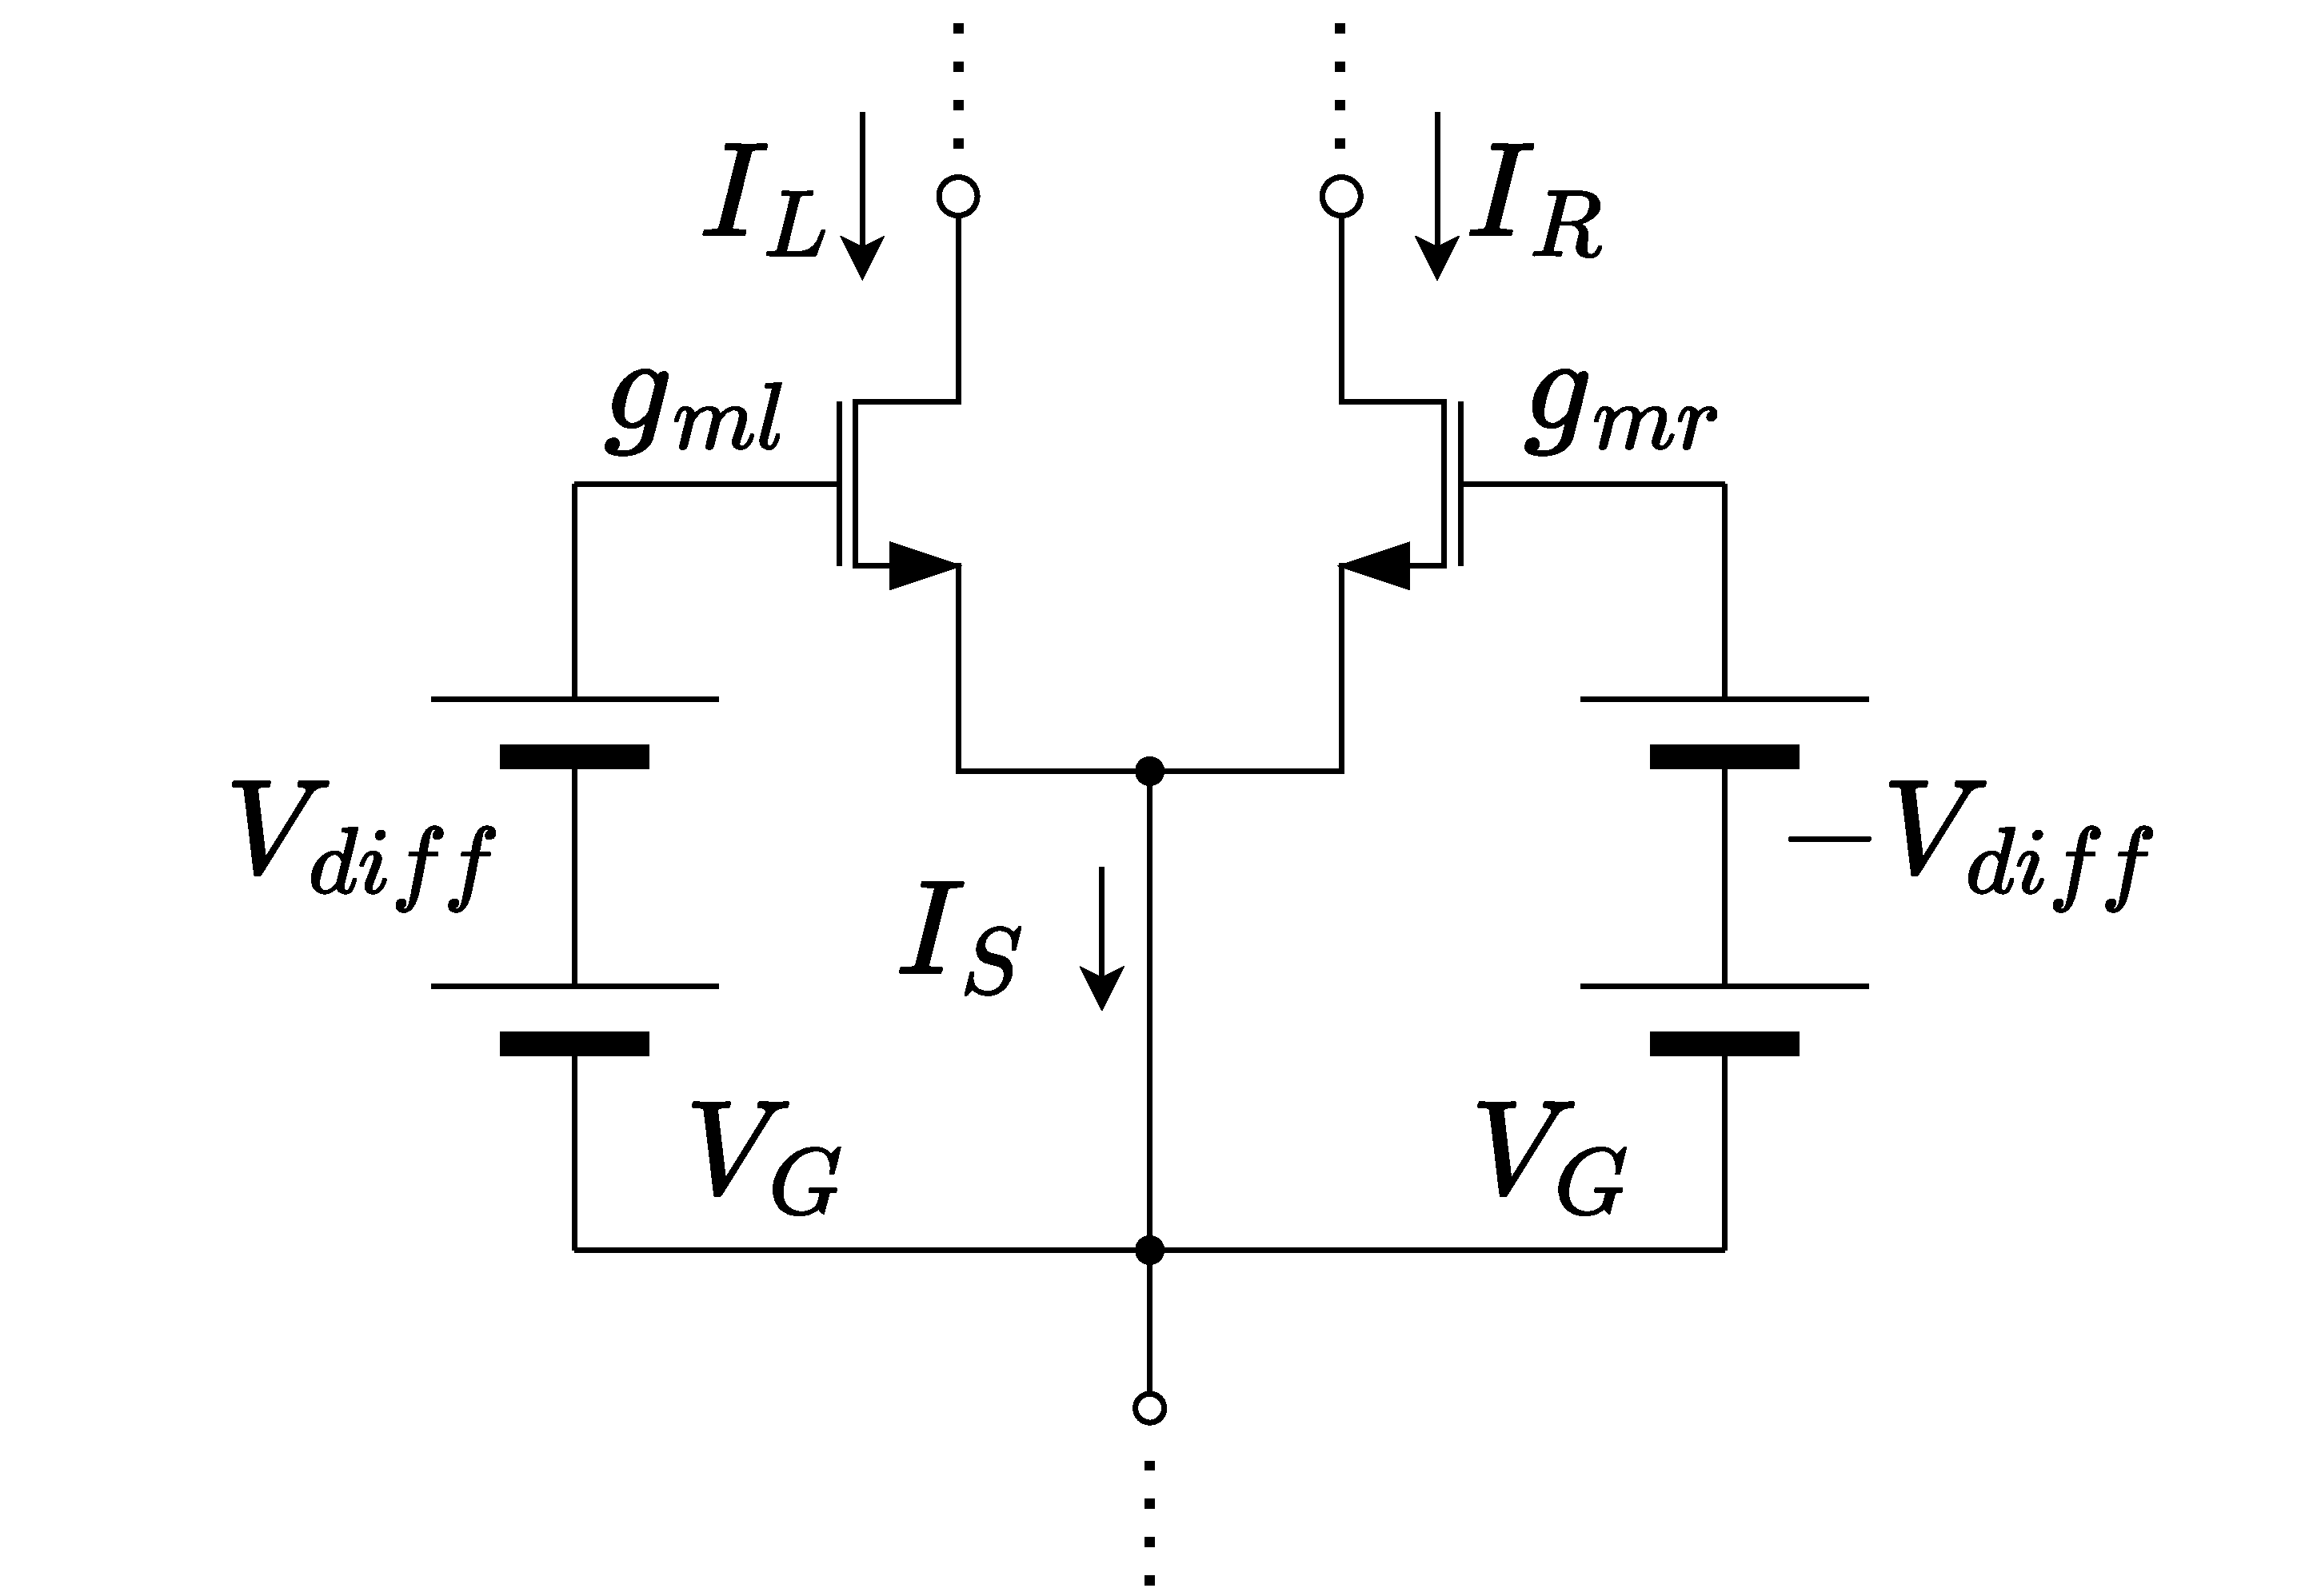
\includegraphics[width=0.5\textwidth]{figures/chapter2/OperatingPoint.pdf}
                    \caption{ゲート接地の差動対}
                    \label{fig:2_OP}
                \end{center}
            \end{figure}
            一般に、MOSFETのドレイン電流は二乗則に従い、ゲートソース間電圧$V_{GS}$、しきい電圧$V_{th}$と形状などによって決まる固有の係数$K$を用いて
            \begin{align}
                I_{D}=K(V_{GS}-V_{th})^{2}  \label{eq:2_id}
            \end{align}
            と表せる。さらに、MOSFETのトランスコンダクタンスはドレイン電流をゲートソース間電圧で偏微分したものであるので差動成分が$0$、つまり$V_{diff}=0$のときトランスコンダクタンスを$g_{m}$とすると式(\ref{eq:2_id})を用いて
            \begin{align}
                g_{m}&=\frac{ \partial I_{D} }{ \partial V_{GS} }   \notag\\
                &=2K(V_{GS}-V_{th})     \label{eq:2_gm}
            \end{align}
            となる。次に差動成分$V_{diff}\neq0$のとき、左右のMOSFETのトランスコンダクタンスは
            \begin{align}
                g_{ml}&=2K\left\{ (V_{G}+V_{diff}) -V_{th} \right\}     \notag\\
                &=g_{m}+2KV_{diff}      \notag\\
                g_{mr}&=2K\left\{ (V_{G}-V_{diff}) -V_{th} \right\}     \notag\\
                &=g_{m}-2KV_{diff}      \notag
            \end{align}
            と計算できるので、$2KV_{diff}\equiv\Delta g_{m}$とおけば
            \begin{align}
                g_{ml}&=g_{m}+\Delta g_{m}   \label{eq:2_dgml}\\
                g_{mr}&=g_{m}-\Delta g_{m}   \label{eq:2_dgmr}
            \end{align}
            と求められた。したがって、ゲート接地増幅回路ではゲート電圧に比例したトランスコンダクタンスを得ることができる。
            \newpage
            
        \subsection{小信号等価回路}
            次に小信号等価回路を考えるが、ここでギルバート乗算回路は差動対の組み合わせでできているため、半回路を考えることで回路全体の小信号解析を行うことができる。
            \begin{figure}[!b]
                \begin{center}

                    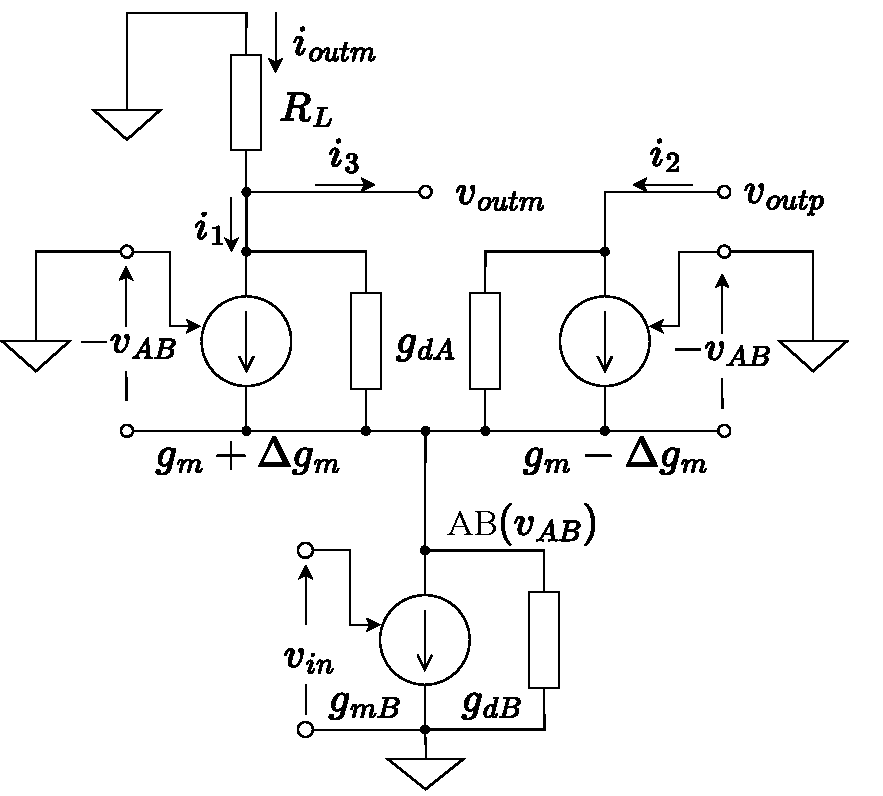
\includegraphics[width=0.99\textwidth]{figures/chapter2/halfeq.pdf}
                    \caption{ギルバート乗算回路の小信号半回路}
                    \label{fig:2_half}

                \end{center}

            \end{figure}
            そこで図\ref{fig:2_gilbert}の$M_{A1},M_{A2},M_{B1}$についての半回路は$V_{S}$が交流的に接地されていることに留意すると、図\ref{fig:2_half}に示すようになる。この時、接点$AB$にKCLを用いると
            \begin{align}
                g_{mB}v_{in}+g_{dB}v_{AB}&=(g_{m}+\Delta g_{m})(-v_{AB})+g_{dA}(v_{outm}-v_{AB})    \notag\\
                &\quad\quad\quad\quad +(g_{m}-\Delta g_{m})(-v_{AB})+g_{dA}(v_{outp}-v_{AB})     \notag\\
                v_{AB}&=-\frac{g_{mB}}{2g_{m}+2g_{dA}+g_{dB}}v_{in}     \label{eq:2_vab}
            \end{align}
            と書ける。さらに、完全差動回路であることを踏まえると$i_{3}=-i_{2}$、$v_{outp}=-v_{outm}$という関係が成り立つ。また最終的な出力電圧を$v_{out}:=v_{outp}-v_{outm}$と定義する。これに留意して負荷抵抗$R_{L}$に流れる電流$i_{outm}$は
            \begin{align}
                i_{outm}&=i_{1}+i_{2}       \notag\\
                &=(g_{m}+\Delta g_{m})(-v_{AB})+g_{dA}(v_{outm}-v_{AB})       \notag\\
                &\quad\quad\quad\quad -\left\{  (g_{m}-\Delta g_{m})(-v_{AB})+g_{dA}(v_{outp}-v_{AB})  \right\}   \notag\\
                &=-2(\Delta g_{m}v_{AB}+g_{dA}v_{out})      \label{eq:2_iout}
            \end{align}
            と表せる。オームの法則を用いると
            \begin{align}
                v_{out}&=\left\{ \left(0-R_{L}i_{outp}\right) - \left(0-R_{L}i_{outm}\right) \right\}    \notag\\
                &=\frac{ 4R_{L} }{1+2R_{L}g_{dA}}\Delta g_{m}v_{AB}     \notag
            \end{align}
            と計算できる。ここで、$g_{m}>>g_{dA},g_{dB}$を仮定し\ref{ch:gilbert_valiable_gm}の結果と式(\ref{eq:2_vab})を用いると出力電圧は
            \begin{align}
                v_{out}=\frac{ 8KR_{L} }{ 1+2R_{L} }\cdot\frac{ g_{mB} }{ 2g_{m} }\cdot V_{CTRL}\cdot v_{in}       \label{eq:2_vout}
            \end{align}
            と表すことができる。ここで、$V_{CTRL}$と$K$はそれぞれ$M_{A}$に与える制御電圧とトランスコンダクタンス係数である。以上より、小信号を入力した際には出力として入力電圧$v_{in}$と制御電圧$V_{CTRL}$に比例した電圧を得る、すなわち乗算ができることが確かめられた。
            \newpage


    \section{出力範囲}
        次にギルバート乗算回路の出力範囲を考える。適切に乗算が行える条件はMOSFETが遮断領域に入らないことであるとすると、制約条件として各MOSFETにおいてしきい電圧$V_{th}$が一定であるとすると
        \begin{subequations}
            \begin{empheq}[left={\empheqlbrace}]{align}
                &V_{GS}-V_{th}<V_{DS}          \\
                &V_{th}<V_{GS}              
            \end{empheq}        \label{eq:2_binding_conditions}
        \end{subequations}
        を満たす必要がある。ただし、$V_{GS}$、$V_{DS}$、$V_{th}$はゲートソース間電圧、ドレインソース間電圧、しきい電圧である。これを図\ref{fig:2_gilbert}の各MOSFETに用いると
        \begin{subequations}
            \begin{empheq}[left={M_{A}:\empheqlbrace}]{align}
                &V_{A}+V_{CTRL}-V_{AB}-V_{th}<V_{out}-\frac{1}{2}v_{out}-V_{AB}           \\
                &V_{th}<V_{A}-V_{CTRL}-V_{AB}                               
            \end{empheq}        \label{eq:2_ma_binding_pre}
        \end{subequations}
        \begin{subequations}
            \begin{empheq}[left={M_{B}:\empheqlbrace}]{align}
                &V_{B}+v_{in}-V_{S}-V_{th}<V_{AB}-V_{S}      \\
                &V_{th}<V_{B}-v_{in}-V_{S}                  
            \end{empheq}        \label{eq:2_mb_binding_pre}
        \end{subequations}
        \begin{subequations}
            \begin{empheq}[left={M_{C}:\empheqlbrace}]{align}
                &V_{C}-V_{th}<V_{S}      \\
                &V_{th}<V_{C}           
            \end{empheq}        \label{eq:2_mc_binding_pre}
        \end{subequations}
        と表現することができる。$M_{A},M_{B}$の.a不等式には両辺にソース電位が含まれているのでそれを消去すると
        \begin{subequations}
            \begin{empheq}[left={M_{A}:\empheqlbrace}]{align}
                &V_{A}+V_{CTRL}-V_{th}<V_{out}-\frac{1}{2}v_{out}           \\
                &V_{th}<V_{A}-V_{CTRL}-V_{AB}                 
            \end{empheq}        \label{eq:2_ma_binding}
        \end{subequations}
        \begin{subequations}
            \begin{empheq}[left={M_{B}:\empheqlbrace}]{align}
                &V_{B}+v_{in}-V_{th}<V_{AB}      \\
                &V_{th}<V_{B}-v_{in}-V_{S}      
            \end{empheq}        \label{eq:2_mb_binding}
        \end{subequations}
        とまとめられる。さらに式(\ref{eq:2_mc_binding_pre})より
        \begin{align}
            0<V_{S}     \label{eq:2_range_vs}
        \end{align}
        である。次に式(\ref{eq:2_ma_binding})から$V_{A}$を消去すると
        \begin{align}
            V_{AB}+2V_{CTRL}<V_{out}-\frac{1}{2}v_{out}     \label{eq:2_range_va}\\
        \end{align}
        であり、また式(\ref{eq:2_mb_binding})から$V_{B}$を消去すると
        \begin{align}
            V_{S}+2v_{in}<V_{AB}        \label{eq:2_range_vb}
        \end{align}
        と分かる。以上より、式(\ref{eq:2_range_va}),(\ref{eq:2_range_va})から
        \begin{align}
            V_{S}+2v_{in}+2V_{CTRL}<V_{out}-\frac{1}{2}v_{out}      \label{eq:2_range_out}
        \end{align}
        である。さらに、出力電圧は電源電圧からも制約を受けるので
        \begin{align}
            V_{out}+v_{out}<V_{dd}
        \end{align}
        であり、出力範囲を$v_{range}$とすると式(\ref{eq:2_range_out})と合わせ
        \begin{align}
            0<v_{range}<V_{dd}-(V_{S}+2V_{CTRL}+2v_{in})    \label{eq:2_girlbert_range}
        \end{align}
        と考えることができる。



%    \begin{figure}
%        \begin{center}
%            \includegraphics[width=125mm]{figures/chapter2}
%            \caption{}
%            \label{fig:2_}
%        \end{center}
%    \end{figure}

%    \begin{subequations}
%        \begin{empheq}[left={\empheqlbrace}]{align}
%        \end{empheq}        \label{eq:}
%    \end{subequations}
